\documentclass[15pt]{report}

%---------Packages---------%
%==========================%
\usepackage{graphicx}
\usepackage{breakurl}
\usepackage{xcolor}

\definecolor{blu}{HTML}{145680} % Custom URL color
\usepackage[colorlinks=true, urlcolor=blu]{hyperref}
%==========================%

\begin{document}
	
%-----------Title-----------%
%===========================%
\definecolor{urlcol}{HTML}{145680}
\title{Handling snow routes in the city of Boston} 

\author{Steven Brzozowski,Chris Joe, Benjamin Kincaid, \and Keith Lovett}
\maketitle
%===========================%

\section*{Introduction}
The city of Boston is notorious for its extreme winter weather. With snowstorms potentially causing problems ranging from minor inconveniences like traffic backup to more serious concerns like roads to hospitals being blocked, it's important to clear snow from roads as efficiently as possible. 

\section*{Problem}
The question that we must solve is: \textit{How do we optimize snow plowing and what will maximize convenience for the city of Boston?} To answer this, we must figure out constraints of the problem and categorize road plowing effectiveness using the datasets we have obtained.

\section*{Datasets}
% traffic signals, snow emergency routes, property assessment
\begin{figure}[h!]
	\centering
	\fbox{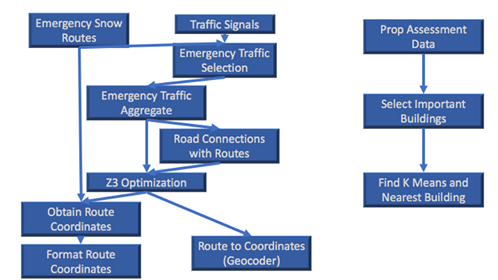
\includegraphics[width=118mm]{Fig_2.png}}
	\caption{Data Flow Diagram}
	\label{fig:method}
\end{figure}
\begin{itemize}
	\item \textbf{Traffic Signals} - a dataset that consists of traffic signals on Boston intersections
	\item \textbf{Snow Emergency Routes} - a dataset of all snow emergency routes and streets affiliated with them
	\item \textbf{Property Assessment} - a dataset that holds buildings and properties with their associated metadata tags.
\end{itemize}

\noindent The datasets used are property assessments from Analyze Boston, traffic signal data and snow emergency routes data from Boston Open Data. Using the snow emergency routes and traffic signal data, we produce the dataset \textbf{emergency\_traffic\_selection} to find traffic signals that are within snow emergency routes. Then we use that selection to aggregate all intersections from the same street on the emergency route. Using the aggregate, we can then find the number of intersections and the routes associated with the street for every street - then finally, we can use our road connections dataset and aggregated emergency traffic dataset to create high priority routes. With the property assessment data, we select important buildings based off of what type of building they are (e.g. hospitals, schools, clinics, supermarkets). We use the important buildings dataset to find a focal point of buildings through k-means clustering. 

\section*{Transformations}
% emergency_traffic_aggregate, emergency_traffic_selection, find_buildings_and_centroids, format_route_coords, obtain_route_coords, road_connections_with_routes, routes_to_coords, select_imp_builds, z3_route_optimization
\begin{itemize}
	\item \textbf{emergency\_traffic\_selection} - Outputs traffic signals that are used within snow emergency routes
	\item \textbf{emergency\_traffic\_aggregate} - Aggregates all intersections from the same street on a snow emergency route
	\item \textbf{selectImpBuilds} - Selects defined important buildings from property data.
	\item \textbf{road\_connections\_with\_routes} - Obtains all roads in Boston region with their connections to other routes
	\item \textbf{z3\_route\_optimization} - returns a list of defined high priority routes using the z3 library and given constraints.
	\item \textbf{find\_buildings\_and\_centroids} - finds k-means clusters and associates closest buildings to the centroids
	\item \textbf{coordinate files} - Retrieves coordinates, formats them, and outputs them in order to use for visualization purposes.
\end{itemize}

\section*{Algorithms and Methods}
% We should talk about k-means clustering too on a high level
To assist in efficient snow removal efforts, we classify the effectiveness of plowing a particular road in two ways: "road priority" and "connections." This is why we manipulated our datasets to include node-like and edge-like representations of our roads. Road priority gauges how much plowing a particular road would benefit traversal throughout the city. At this stage of the project we are gauging this based on emergency snow routes. We will define a "high priority set" as a subset of Boston's emergency snow routes in which all other streets have access to at least one emergency route. We optimize this by finding the high priority set with the fewest emergency routes possible. "Connections" gauge how plowing a particular road would benefit access to nearby buildings of importance, and is optimized via a run of the K-means algorithm, wherein clusters to be closed in on by K-means are defined by the coordinates of these buildings of importance. We then perform analysis of the K-means result to return the distance to the nearest centroid for each point of importance.
In our visualization, the K-means result is displayed alongside the constraint satisfaction result. Roads to be prioritized by the city to plow first, are those with the smallest distance between them, and the nearest centroid.

%Usage, tools, efficiency
\section*{Usage, Adjustments, Performance}
\subsection*{Performance}
The project itself is rather lightweight since most of the raw code is executed with minimal dependencies. The Python code depends on the following libraries: \textbf{numpy, scipy, sklearn, z3-solver}. However, the datasets derived from \textbf{Boston Open Data} and \textbf{Analyze Boston} range from medium-sized (couple thousand points) to large-sized (hundreds of thousands of points). Due to this, the speed of running the entire set of algorithms is discernible: the process takes anywhere from three to five minutes. When running the trial mode of the algorithm (\textbf{-{}-trial}), it takes considerably less time, though this is due to taking less samples from our datasets so accuracy may vary. From this, we realize that our speed is gated by how fast we can process a large dataset - at its slowest, it is around O(n$^2$) from what we can compute. However, \textbf{z3 optimization} does not have a numerical time complexity because it brute forces acceptable solutions given our constraints. This still runs in a reasonable amount of time, due to the fact that \textbf{z3} creates optimizations to run the algorithm. The details of the optimizations are black-boxed so we cannot infer the exact running time. The visualization used to take a long time to be generated when we overlay the map with markers. This is in part due to limitations on the standard usage limits of Google Maps' geocoder API, which allows for a limited number of queries per second. However, we have decided to keep an array of coordinates that correspond to routes in Boston for the sake of speeding up our runtime. Now, during runtime, we call the array to create our routes dynamically instead of doing rate-limited calls to Google's geocoder. 

%For this reason we have allowed the user to enable/disable the generation of markers, so that  without markers generated, they can still view a very lightweight and fast visualization that is informative of what routes of the city could be plowed first. We have also allowed the user to track the progress of the generation of their markers via the terminal window running server.py.

\subsection*{Adjustments}
The datasets needed little adjustments to be compatible with our project. In terms of raw transformations, we frequently used selections to filter our the necessary data we needed, and then aggregated certain data in order to feed desired information into our algorithms. We are constrained by some particular datasets - for example, we do not have every single street in Boston but rather most of them. However, we are able to mitigate this by establishing road connections until we are able to be sure that every route can be connected to every possible road inside our dataset. The algorithm is correct within our dataset but may not necessarily be one hundred percent accurate should it be compared against a dataset that has every road, major or minor, in Boston. Furthermore, when visualizing the project, we require a minimum of 112 routes to be visualized because the problem is not satisfiable unless we have a minimum of 112 routes. We also require a maximum of 144 routes, if only because Boston has 144 usable routes in total. 

\section*{Results}
\begin{figure}[h!]
	\centering
	\fbox{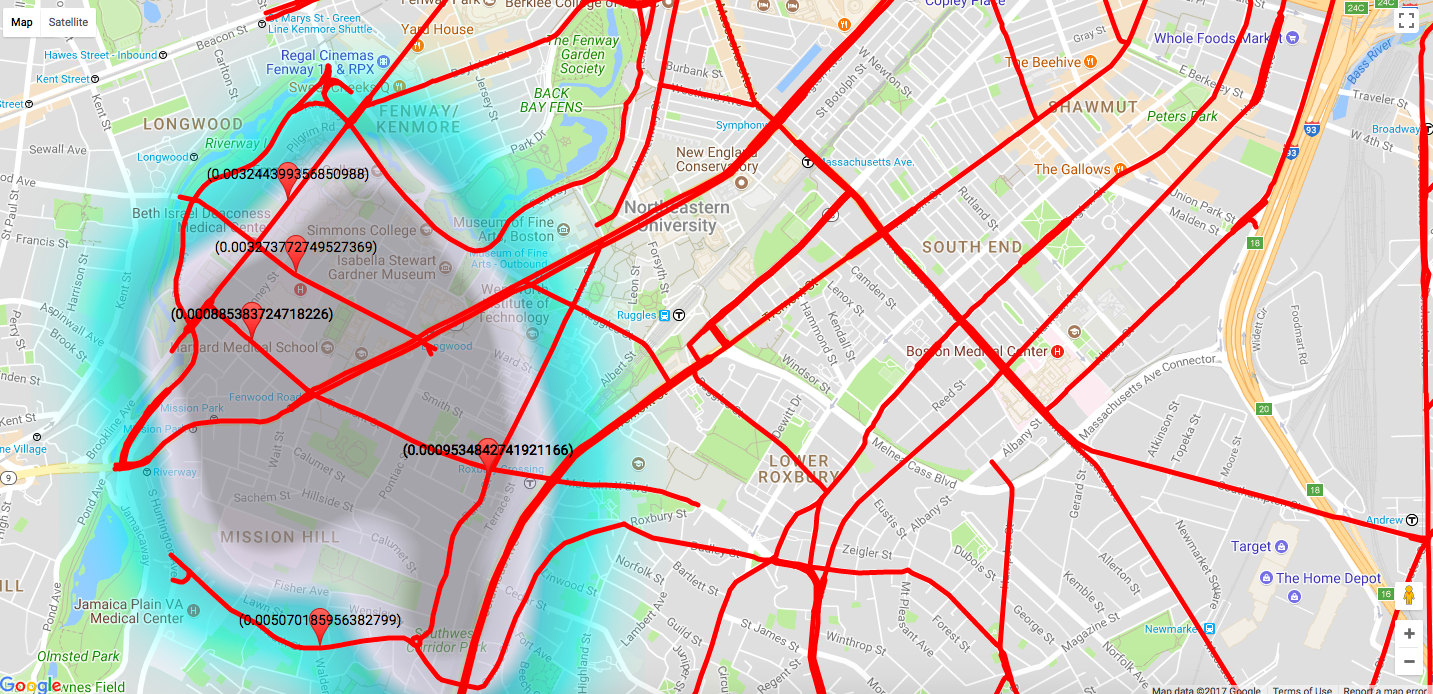
\includegraphics[width=118mm]{updatedFigure.png}}
	\caption{Heatmaps with Priority Roads}
	\label{fig:method}
\end{figure} 
\noindent Using the datasets obtained, we plot our results to the map of Boston. First, we use our \textbf{z3-optimization} to plot the minimum amount of high-priority routes that are necessary to reach every street in Boston. Then, we build a heatmap based on our solution to the K-means clustering of important buildings (e.g. hospitals, clinics, schools, etc). These heatmaps show areas where there are higher densities of buildings that need to be prioritized.

\section*{Conclusion}
Using both results (the heatmap and high-priority roads), we are able to infer which streets should be plowed first by associating the two together. This means that, for every high-priority road, it should be also be given a weight that is based off of its availability and distance to the area of the heatmaps provided. \\\\
%\hrule
\pagebreak
\section*{Sources}
\sloppy 
\textbf{Traffic Signals} \\
\url{http://bostonopendata-boston.opendata.arcgis.com/datasets/de08c6fe69c942509089e6db98c716a3_0.geojson} \\\\
\textbf{Snow Emergency Routes} \\
\url{http://bostonopendata-boston.opendata.arcgis.com/datasets/4f3e4492e36f4907bcd307b131afe4a5_0.geojson} \\\\
\textbf{Property Assessment} \\
\url{https://data.boston.gov/api/3/action/datastore_search?resource_id=cecdf003-9348-4ddb-94e1-673b63940bb8}

\end{document}